\section{The Reinforcement Learning (RL) setting}


\definecolor{reward}{rgb}{0,0.5,0}
\definecolor{policy}{rgb}{0.75,0,0}
\definecolor{trans}{rgb}{0,0,1}

\begin{frame}\frametitle{\secname}

\only<1>{
Reminder:
\begin{itemize}
\item Data in supervised learning:
$
\Big\{
	\vec x^{(\alpha)} \in \R^N
	\,,\,
	\vec y_T^{(p)} \in \R^M
\Big\}_{\alpha=1}^{p}
$

\item Data in \textbf{un}supervised learning:
$
\Big\{
	\vec x^{(\alpha)} \in \R^N
\Big\}_{\alpha=1}^{p}
$\\

\end{itemize}
}

\only<1->{
Data in Reinforcement Learning:
}
\only<1>{
\begin{itemize}
	\item[] A sequence of random states $\vec x$
	\item[] resulting from taking actions $\vec a$ over time
	\item[] which result in some reward $r$.
\end{itemize}
}
\pause
\only<2->{
\begin{itemize}
\item a state $\vec x \in \mathcal{X}$ or $\vec x \in \R^N$,\\
e.g. $\mathcal{X} := \{ \vec x_1, \ldots, \vec x_S\} \subset \{0,1\}^S$ (1-out-$S$ encoding)
\pause
\item an action $\vec a$ which can be taken by the agent:\\

$\vec a \in \mathcal{A}$ or $\vec a \in \R^M$,\\
 e.g. $\mathcal{A} := \{ \vec a_1, \ldots, \vec a_A\} \subset \{0,1\}^A$ (1-out-$A$ encoding)
\pause
\item a reward $r \in \R$ or $r \in \{0,1\}$,\\
 e.g. $r \in \{\text{``cheese''},\text{``no cheese''}\}$.

\end{itemize}
\pause
\mode<article>{Each time step describes what reward was received when performing some action while in some state. 
}
The sequence we observe becomes:

\slidesonly{\vspace{-4mm}}

\begin{align}
\label{eq:chain}
\left\{\vec x^{(t)}, \vec a^{(t)}, r^{(t)}\right\}_{t=0}^{p} = 
\left( \vec x^{(0)}, \vec a^{(0)}, r^{(0)} \right) \,,\, \ldots \,,\, \left(\vec x^{(p)}, \vec a^{(p)}, r^{(p)} \right)
\end{align}
}

\end{frame}

\subsection{The Transition Model}

\begin{frame}

\only<1,2>{    
\begin{block}{Markov property}

The probability of transitioning from state $\vec x_i$ to $\vec x_j$ only depends on state $\vec x_i$ and the action $\vec a_k$ that was taken. It does not depend on earlier history.
\end{block}
}
\only<2-4>{
This leads to the following \textcolor{trans}{transition model (transition ``matrix'')}:

\svspace{-3mm}

\begin{equation}
{
\color{trans}
P(\vec x_j | \vec x_i, \vec a_k)
}
\end{equation}

\only<2->
{
which
\begin{itemize}
	\item measures the probability to end up in $\vec x_j$ 
		after choosing $\vec a_k$ when in $\vec x_i$,
	\item is a stationary distribution
	\begin{equation}
	P(\vec x_j^{(t+1+\tau)} | \vec x_i^{(t+\tau)}, \vec a_k^{(t+\tau)}) = P(\vec x_j^{(t+1)} | \vec x_i^{(t)}, \vec a_k^{(t)})\,,\quad \tau \in \{0,1,\ldots\}
	\end{equation}
\end{itemize}
}
\only<3>{
\mode<presentation>{
	\begin{center}
		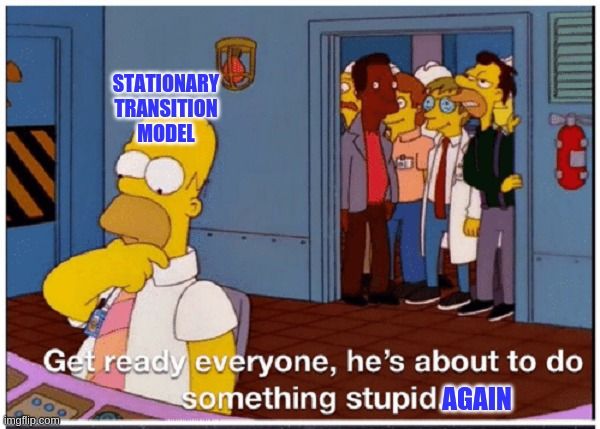
\includegraphics[width=0.3\textwidth]{img/meme_stationary}
	\end{center}
	}
}
\only<4>{

and where
\begin{align}
{\color{trans}P(\vec x_j | \vec x_i, \vec a_k)} &\ge 0 \quad \forall i,j,k\\
\text{and}~ \sum_{j} {\color{trans}P(\vec x_j | \vec x_i, \vec a_k)} &= 1 \quad \forall i,k \quad \text{i.e. every ``row'' sums to 1}
\end{align}
}
}

\end{frame}

\begin{frame}{Properties of the transition model}

\svspace{-4mm}

\question{What would $\sum_{\substack{j\\j \ne i}} {P(\vec x_j | \vec x_i, \vec a_k)} = 0 \;\; \forall \; k$ imply?}

\pause

\slidesonly{\vspace{-3mm}}
- $\vec x_i$ \notesonly{is a state which leads nowhere else, regardless of the action. It }is a \emph{terminal state}.

\question{What does an entry ${P(\vec x_j | \vec x_i, \vec a_k)} = 0$ represent?}

\pause

- When at $\vec x_i$, taking action $\vec a_k$ can never lead to $\vec x_j$.


\question{What does an entry ${P(\vec x_j | \vec x_i, \vec a_k)} = 0 \;\; \forall \; k$ represent?}

\pause

- It is impossible to go from $\vec x_i$ to $\vec x_j$, regardless of the action.

\question{What does an entry ${P(\vec x_j | \vec x_i, \vec a_k)} = 1$ represent?}

\pause

- When at $\vec x_i$, taking action $\vec a_k$ always leads to $\vec x_j$.

\end{frame}

\begin{frame}

\mode<presentation>{
\textcolor{trans}{transition model (transition matrix)}:

\begin{equation}
{
\color{trans}
P(\vec x_j | \vec x_i, \vec a_k)
}
\end{equation}
}

\begin{block}{Markov chain}
a sequence of random states $\vec x$ with a \emph{Markov property}.
\end{block}


\end{frame}

\subsection{The Policy}

\begin{frame}

\begin{block}{\textcolor{policy}{Policy}}
Representation of the agent\footnote{
Without a policy we would only have a Markov Reward Process.
Having a policy (wanting to find a policy) turns the Markov Reward Process into a Markov Decision Process.
}. It measures the distribution over actions given states.
\begin{itemize}
\item map states to actions, i.e. the probability of doing $\vec a_k$ when in $\vec x_i$:

\begin{equation}
\color{policy}
\text{policy }\pi := \pi(\vec a_k | \vec x_i)
\end{equation}

\pause

\item the mapping can be stochastic or deterministic
\item the policy is stationary. That the policy changes during the training process does not contradict this.
It is regarded as stationary because once trained and deployed, the way the agent decides does not change over time.
\end{itemize}

\end{block}

\end{frame}
